

\chapter{Nose cone and transition geometries}
\label{app-nosecone-geometry}

Model rocket nose cones are available in a wide variety of shapes and
sizes.  In this appendix the most common shapes and their defining
parameters are presented.


\section{Conical}

The most simple nose cone shape is a right circular cone.  They are
easy to make from a round piece of cardboard.  A conical nose cone is
defined simply by its length and base diameter. An additional
parameter is the opening angle $\phi$, shown in
Figure~\ref{fig-nosecone-shapes}(a).  The defining equation of a
conical nose cone is
%
\begin{equation}
r(x) = \frac{x}{L}\cdot R.
\end{equation}


\section{Ogival}

Ogive nose cones have a profile which is an arc of a circle, as shown
in Figure~\ref{fig-nosecone-shapes}(b).  The most common ogive shape
is the {\it tangent ogive} nose cone, which is formed when radius of
curvature of the circle $\rho_t$ is selected such that the joint
between the nose cone and body tube is smooth,
%
\begin{equation}
\rho_t = \frac{R^2+L^2}{2R}.
\end{equation}
%
If the radius of curvature $\rho$ is greater than this, then the
resulting nose cone has an angle at the joint between the nose cone
and body tube, and is called a {\it secant ogive}.  The secant ogives
can also be viewed as a larger tangent ogive with its base cropped.
At the limit $\rho\rightarrow\infty$ the secant ogive becomes a
conical nose cone.

The parameter value $\kappa$ used for ogive nose cones is the ratio of
the radius of curvature of a corresponding tangent ogive $\rho_t$ to
the radius of curvature of the nose cone $\rho$:
%
\begin{equation}
\kappa = \frac{\rho_t}{\rho}
\end{equation}
%
$\kappa$ takes values from zero to one, where $\kappa=1$ produces a
tangent ogive and $\kappa=0$ produces a conical nose cone (infinite
radius of curvature).

With a given length $L$, radius $R$ and parameter $\kappa$ the radius
of curvature is computed by
%
\begin{equation}
\rho^2 = \frac{ \del{L^2+R^2}\cdot
  \del{ \del{\del{2-\kappa}L}^2 + \del{\kappa R}^2 }
}{ 4\del{\kappa R}^2 }.
\end{equation}
%
Using this the radius at position $x$ can be computed as
%
\begin{equation}
r(x) = \sqrt{\rho^2 - \del{L/\kappa - x}^2} - \sqrt{\rho^2-\del{L/\kappa}^2}
\end{equation}



\section{Elliptical}

Elliptical nose cones have the shape of an ellipsoid with one major
radius is $L$ and the other two $R$.  The profile has a shape of a
half-ellipse with major axis $L$ and $R$,
Figure~\ref{fig-nosecone-shapes}(c).  It is a simple geometric shape
common in model rocketry.  The special case $R=L$ corresponds to a
half-sphere.

The equation for an elliptical nose cone is obtained by stretching the
equation of a unit circle:
\begin{equation}
r(x) = R \cdot \sqrt{1-\del{1-\frac{x}{L}}^2}
\end{equation}


\section{Parabolic series}

A parabolic nose cone is the shape generated by rotating a section of
a parabola around a line perpendicular to its symmetry axis,
Figure~\ref{fig-nosecone-shapes}(d).  This is
distinct from a paraboloid, which is rotated around this symmetry
axis (see Appendix~\ref{app-power-series}).  

Similar to secant ogives, the base of a ``full'' parabolic nose cone
can be cropped to produce nose cones which are not tangent with the
body tube.  The parameter $\kappa$ describes the portion of the larger
nose cone to include, with values ranging from zero to one.  The most
common values are $\kappa=0$ for a conical nose cone, $\kappa=0.5$ for
a 1/2~parabola, $\kappa=0.75$ for a 3/4~parabola and $\kappa=1$ for a
full parabola.  The equation of the shape is
%
\begin{equation}
r(x) = R\cdot\frac{x}{L} \del{ \frac{2 - \kappa\frac{x}{L}}
   {2-\kappa}}.
\end{equation}



\section{Power series}
\label{app-power-series}

The power series nose cones are generated by rotating the segment
%
\begin{equation}
r(x) = R\del{\frac{x}{L}}^\kappa
\end{equation}
%
around the x-axis, Figure~\ref{fig-nosecone-shapes}(e).  The parameter
value $\kappa$ can range from zero to one.  Special cases are
$\kappa=1$ for a conical nose cone, $\kappa=0.75$ for a 3/4~power nose
cone and $\kappa=0.5$ for a 1/2~power nose cone or an ellipsoid.
The limit $\kappa\rightarrow0$ forms a blunt cylinder.


\section{Haack series}

In contrast to the other shapes which are formed from rotating
geometric shapes or simple formulae around an axis, the Haack series
nose cones are mathematically derived to minimize the theoretical
pressure drag.  Even though they are defined as a series, two specific
shapes are primarily used, the {\it LV-Haack}\ shape and the 
{\it LD-Haack}\ or {\it Von K�rman}\ shape.  The letters LV and LD
refer to length-volume and length-diameter, and they minimize the
theoretical pressure drag of the nose cone for a specific length and
volume or length and diameter, respectively.  Since the parameters
defining the dimensions of the nose cone are its length and radius,
the Von K�rman nose cone (Figure~\ref{fig-nosecone-shapes}(f)) should,
in principle, be the optimal nose cone shape.

The equation for the series is
%
\begin{equation}
r(x) = \frac{R}{\sqrt{\pi}} \;
  \sqrt{\theta - \frac{1}{2}\sin(2\theta) + \kappa \sin^3\theta}
\end{equation}
%
where
%
\begin{equation}
\theta = \cos^{-1} \del{1-\frac{2x}{L}}.
\end{equation}
%
The parameter value $\kappa=0$ produces the Von K�rman of LD-Haack
shape and $\kappa=1/3$ produces the LV-Haack shape.  In principle,
values of $\kappa$ up to $2/3$ produce monotonic nose cone shapes.
However, since there is no experimental data available for the
estimation of nose cone pressure drag for $\kappa > 1/3$ (see
Appendix~\ref{app-haack-series-pressure-drag}), the selection of the
parameter value is limited in the software to the range 
$0 \ldots 1/3$.


\section{Transitions}

The vast majority of all model rocket transitions are conical.
However, all of the nose cone shapes may be adapted as transition
shapes as well.  The transitions are parametrized with the fore and
aft radii $R_1$ and $R_2$, length $L$ and the optional shape parameter
$\kappa$.

Two choices exist when adapting the nose cones as transition shapes.
One is to take a nose cone with base radius $R_2$ and crop the tip of
the nose at the radius position $R_1$.  The length of the nose cone
must be selected suitably that the length of the transition is $L$.
Another choice is to have the profile of the transition resemble two
nose cones with base radius $R_2-R_1$ and length $L$.  These two
adaptations are called {\it clipped} and {\it non-clipped} transitions,
respectively.  A clipped and non-clipped elliptical transition is
depicted in Figure~\ref{fig-transition-clip}.

For some transition shapes the clipped and non-clipped adaptations are
the same.  For example, the two possible ogive transitions have equal
radii of curvature and are therefore the same.  Specifically, the
conical and ogival transitions are equal whether clipped or not, and
the parabolic series are extremely close to each other.




\begin{figure}[p]
\centering
\begin{tabular}{ccc}

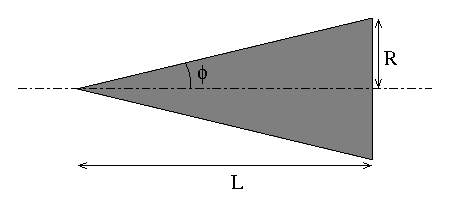
\epsfig{file=figures/nose-geometry/geometry-conical,scale=0.7} &&
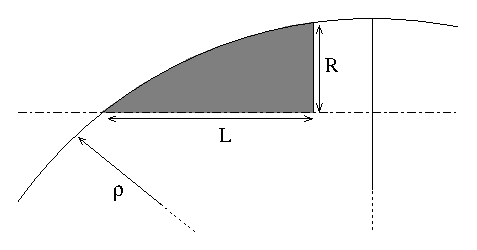
\epsfig{file=figures/nose-geometry/geometry-ogive,scale=0.7} \\
(a) & \hspace{1cm} & (b) \\
&& \\
&& \\
&& \\
%&& \\

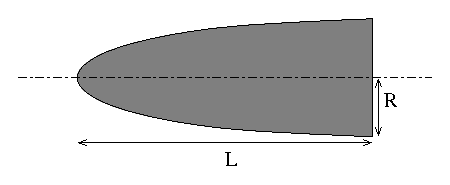
\epsfig{file=figures/nose-geometry/geometry-elliptical,scale=0.7} &&
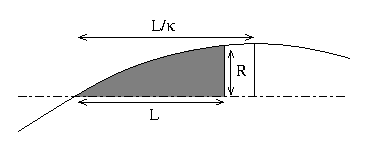
\epsfig{file=figures/nose-geometry/geometry-parabolic,scale=1.0} \\
(c) && (d) \\
&& \\
&& \\
&& \\
%&& \\

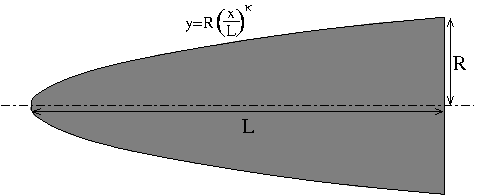
\epsfig{file=figures/nose-geometry/geometry-power,scale=0.6} &&
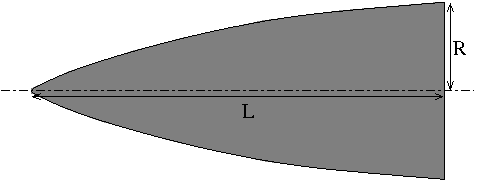
\epsfig{file=figures/nose-geometry/geometry-haack,scale=0.6} \\
(e) && (f) \\
&& \\
%&& \\
\end{tabular}
\caption{Various nose cone geometries:  (a)~conical, (b)~secant ogive,
  (c)~elliptical, (d)~parabolic, (e)~1/2~power (ellipsoid) and
  (f)~Haack series (Von K�rman).}
\label{fig-nosecone-shapes}
\end{figure}

\begin{figure}[p]
\vspace{5mm}
\begin{center}
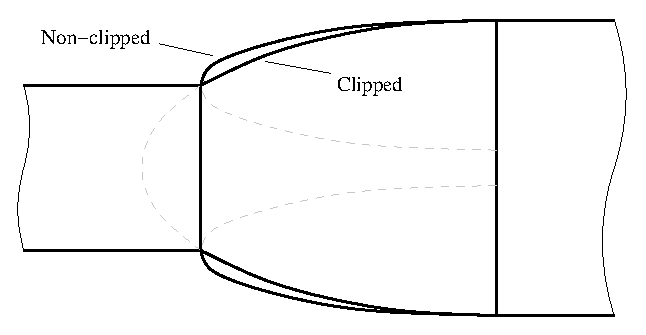
\epsfig{file=figures/nose-geometry/geometry-transition,scale=0.7}
\end{center}
\caption{A clipped and non-clipped elliptical transition.}
\label{fig-transition-clip}
\end{figure}





\chapter{Transonic wave drag of nose cones}
\label{app-nosecone-drag-method}

The wave drag of different types of nose cones vary largely in the
transonic velocity region.  Each cone shape has its distinct
properties.  In this appendix methods for calculating and
interpolating the drag of various nose cone shapes at transonic and
supersonic speeds are presented.  A summary of the methods is
presented in Appendix~\ref{app-transonic-nosecone-summary}.



\section{Blunt cylinder}
\label{app-blunt-cylinder-drag}

A blunt cylinder is the limiting case for every nose cone shape at the
limit $f_N\rightarrow 0$.  Therefore it is useful to have a formula
for the front pressure drag of a circular cylinder in longitudinal
flow.  As the object is not streamline, its drag coefficient does not
vary according to the Prandtl factor~(\ref{eq-prandtl-factor}).
Instead, the coefficient is approximately proportional to the
{\it stagnation pressure}, or the pressure at areas perpendicular to
the airflow.  The stagnation pressure can be approximated by the
function~\cite[pp.~15-2,~16-3]{hoerner}
%
\begin{equation}
\frac{q_{\rm stag}}{q} =
\left\{
\begin{array}{ll}
1 + \frac{M^2}{4} + \frac{M^4}{40}, & \mbox{for\ } M < 1 \\
1.84 - \frac{0.76}{M^2} + \frac{0.166}{M^4} + \frac{0.035}{M^6}, &
   \mbox{for\ } M > 1
\end{array}
\right. .
\end{equation}
%
The pressure drag coefficient of a blunt circular cylinder as a
function of the Mach number can then be written as
%
\begin{equation}
(C_{D\bullet})_{\rm pressure} = 
(C_{D\bullet})_{\rm stag} = 0.85 \cdot \frac{q_{\rm stag}}{q}.
\label{eq-blunt-cylinder-drag}
\end{equation}





\section{Conical nose cone}

A conical nose cone is simple to construct and closely resembles many
slender nose cones.  The conical shape is also the limit of several
parametrized nose cone shapes, in particular the secant ogive with
parameter value 0.0 (infinite circle radius), the power series nose
cone with parameter value 1.0 and the parabolic series with parameter
value 0.0.

Much experimental data is available on the wave drag of conical nose
cones.  Hoerner presents formulae for the value of $C_{D\bullet}$ at
supersonic speeds, the derivative  $\dif C_{D\bullet}/\dif M$ at
$M=1$,  and a figure of $C_{D\bullet}$ at
$M=1$~\cite[pp.~16-18\ldots16-20]{hoerner}.  Based on these and 
the low subsonic drag coefficient~(\ref{eq-nosecone-pressure-drag}), a
good interpolation of the transonic region is possible.

The equations presented by Hoerner are given as a function of the
half-apex angle $\varepsilon$, that is, the angle between the conical
body and the body centerline.  The half-apex angle is related to the
nose cone fineness ratio by
%
\begin{equation}
\tan\varepsilon = \frac{d/2}{l} = \frac{1}{2f_N}.
\end{equation}

The pressure drag coefficient at supersonic speeds ($M\gtrsim1.3$) is
given by
%
\begin{align}
(C_{D\bullet})_{\rm pressure}
& =  2.1\;\sin^2\varepsilon + 0.5\;
                 \frac{\sin\varepsilon}{\sqrt{M^2-1}} \nonumber\\
& =  \frac{2.1}{1+4f_N^2} + \frac{0.5}{\sqrt{(1+4f_N^2)\; (M^2-1)}} .
\label{eq-conical-supersonic-drag}
\end{align}
%
It is worth noting that as the Mach number increases, the drag
coefficient tends to the constant value $2.1\sin^2\epsilon$.  At $M=1$
the slope of the pressure drag coefficient is equal to
%
\begin{equation}
\eval{\frac{\partial (C_{D\bullet})_{\rm pressure}}{\partial M}}_{M=1} =
  \frac{4}{\gamma+1} \cdot (1-0.5\;C_{D\bullet,M=1})
\label{eq-conical-sonic-drag-derivative}
\end{equation}
%
where $\gamma=1.4$ is the specific heat ratio of air and the drag
coefficient at $M=1$ is approximately
%
\begin{equation}
C_{D\bullet,M=1} = 1.0\; \sin\varepsilon.
\label{eq-conical-sonic-drag}
\end{equation}

The pressure drag coefficient between Mach~0 and Mach~1 is
interpolated using equation~(\ref{eq-nosecone-pressure-drag}).  
Between Mach~1 and Mach~1.3 the coefficient is calculated using
polynomial interpolation with the boundary conditions from
equations~(\ref{eq-conical-supersonic-drag}),
(\ref{eq-conical-sonic-drag-derivative}) and
(\ref{eq-conical-sonic-drag}).






\section{Ellipsoidal, power, parabolic and Haack series nose cones}
\label{app-haack-series-pressure-drag}

A comprehensive data set of the pressure drag coefficient for all nose
cone shapes at all fineness ratios at all Mach numbers is not
available.  However, Stoney has collected a compendium of nose cone
drag data including data on the effect of the fineness ratio $f_N$ on
the drag coefficient and an extensive study of drag coefficients of
different nose cone shapes at fineness ratio
3~\cite{nosecone-cd-data}.  The same report suggests that the effects 
of fineness ratio and Mach number may be separated.

The curves of the pressure drag coefficient as a function of the nose
fineness ratio $f_N$ can be closely fitted with a function of the form
%
\begin{equation}
(C_{D\bullet})_{\rm pressure} = \frac{a}{(f_N + 1)^b}.
\label{eq-fineness-ratio-drag-interpolator}
\end{equation}
%
The parameters $a$ and $b$ can be calculated from two data points
corresponding to fineness ratios 0 (blunt cylinder,
Appendix~\ref{app-blunt-cylinder-drag}) and ratio 3.  Stoney includes
experimental data of the pressure drag coefficient as a function of
Mach number at fineness ratio 3 for power series $x^{1/4}$, $x^{1/2}$,
$x^{3/4}$ shapes, $1/2$, $3/4$ and full parabolic shapes, ellipsoidal,
L-V~Haack and Von K�rman nose cones.  These curves are written into
the software as data curve points.  For parametrized nose cone shapes
the necessary curve is interpolated if 
necessary.  Typical nose cones of model rockets have fineness ratios
in the region of 2--5, so the extrapolation from data of fineness
ratio 3 is within reasonable bounds.





\section{Ogive nose cones}

One notable shape missing from the data in Stoney's report are secant
and tangent ogives.  These are common shapes for model rocket nose
cones.  However, no similar experimental data of the pressure drag as
a function of Mach number was found for ogive nose cones.

At supersonic velocities the drag of a tangent ogive is approximately
the same as the drag of a conical nose cone with the same length and
diameter, while secant ogives have a somewhat smaller
drag~\cite[p.~239]{handbook-supersonic-aerodynamics}.  The minimum
drag is achieved when the secant ogive radius is approximately twice
that of a corresponding tangent ogive, corresponding to the parameter
value 0.5.  The minimum drag is consistently 18\% less than that of a
conical nose at Mach numbers in the range of 1.6--2.5 and for fineness
ratios of 2.0--3.5.  Since no better transonic data is available, it
is assumed that ogives follow the conical drag profile through
the transonic and supersonic region.  The drag of the corresponding
conical nose is diminished in a parabolic fashion with the ogive
parameter, with a minimum of -18\% at a parameter value of 0.5.





\section{Summary of nose cone drag calculation}
\label{app-transonic-nosecone-summary}

The low subsonic pressure drag of nose cones is calculated using
equation~(\ref{eq-nosecone-pressure-drag}):
%
\begin{equation*}
(C_{D\bullet,M=0})_p = 0.8 \cdot \sin^2\phi.
\end{equation*}
%
The high subsonic region is interpolated using a function of the form
presented in equation~(\ref{eq-nosecone-pressure-interpolator}):
%
\begin{equation*}
(C_{D\bullet})_{\rm pressure} = a\cdot M^b + (C_{D\bullet,M=0})_p
\end{equation*}
%
where $a$ and $b$ are selected according to the lower boundary of the
transonic pressure drag and its derivative.

The transonic and supersonic pressure drag is calculated depending on
the nose cone shape as follows:
%
\begin{itemize}

\item[\bf Conical:]  At supersonic velocities ($M > 1.3$) the
  pressure drag is calculated using
  equation~(\ref{eq-conical-supersonic-drag}).  Between Mach 1 and 1.3
  the drag is interpolated using a polynomial with boundary conditions
  given by equations~(\ref{eq-conical-supersonic-drag}),
  (\ref{eq-conical-sonic-drag-derivative}) and
  (\ref{eq-conical-sonic-drag}).
\\



\item[\bf Ogival:]  The pressure drag at transonic and supersonic
  velocities is equal to the pressure drag of a conical nose cone with
  the same diameter and length corrected with a shape factor:
%, multiplied by the shape factor
%
\begin{equation}
(C_{D\bullet})_{\rm pressure} = 
\del{0.72 \cdot (\kappa - 0.5)^2 + 0.82} \cdot 
(C_{D\bullet})_{\rm cone}.
\end{equation}
%
The shape factor is one at $\kappa = 0, 1$ and 0.82 at $\kappa=0.5$.
\\



\item[\bf Other shapes:]  The pressure drag calculation is based on
  experimental data curves:
%
\begin{enumerate}
\item Determine the pressure drag $C_3$ of a similar nose cone
  with fineness ratio $f_N=3$ from experimental data.  If data for a
  particular shape parameter is not available, interpolate the data
  between parameter values.

\item Calculate the pressure drag of a blunt cylinder $C_0$
  using equation~(\ref{eq-blunt-cylinder-drag}).

\item Interpolate the pressure drag of the nose cone using
  equation~(\ref{eq-fineness-ratio-drag-interpolator}).
  After parameter substitution the equation takes the form
%
\begin{equation}
(C_{D\bullet})_{\rm pressure} \;=\;
\frac{C_0}{(f_N+1)^{\log_4 C_0/C_3}} \;=\;
C_0 \cdot \del{\frac{C_3}{C_0}}^{\log_4(f_N+1)}
\end{equation}
%
  The last form is computationally more efficient since the exponent
  $\log_4(f_N+1)$ is constant during a simulation.

\end{enumerate}

\end{itemize}











\chapter{Streamer drag coefficient estimation}
\label{app-streamers}


A streamer is a typically rectangular strip of plastic or other
material that is used as a recovery device especially in small model
rockets.  The deceleration is based on the material flapping in the
passing air, thus causing air resistance.  Streamer optimization has
been a subject of much interest in the rocketry
community~\cite{streamer-optimization}, and contests on streamer
landing duration are organized regularly.  In order to estimate the
drag force of a streamer a series of experiments were performed and an
empirical formula for the drag coefficient was developed.

One aspect that is not taken into account in the present investigation
is the fluctuation between the streamer and rocket.  At one extreme a
rocket with a very small streamer drops head first to the ground with
almost no deceleration at all.  At the other extreme there is a very
large streamer creating significant drag, and the rocket falls below
it tail-first.  Between these two extremes is a point where the
orientation is labile, and the rocket as a whole twirls
around during descent.  This kind of interaction between the rocket
and streamer cannot be investigated in a wind tunnel and would require
an extensive set of flight tests to measure.  Therefore it is not
taken into account, instead, the rocket is considered effectively a
point mass at the end of the streamer, the second extreme mentioned
above.


\subsubsection*{Experimental methods}

A series of experiments to measure the drag coefficients of streamers
was performed using the $40\times40\times120$~cm wind tunnel of
Pollux~\cite{pollux-wind-tunnel}.  The experiments were performed
using various materials, widths and lengths of streamers and at
different wind speeds.  The effect of the streamer size and shape was
tested separately from the effect of the streamer material.

A tube with a rounded $90^\circ$ angle at one end was installed in the
center of the wind tunnel test section.  A line was drawn through the
tube so that one end of the line was attached to a the streamer and the
other end to a weight which was placed on a digital scale.  When the
wind tunnel was active the force produced by the streamer was read
from the scale.  A metal wire was taped to the edge of the streamer to
keep it rigid and the line attached to the midpoint of the wire.

A few different positions within the test section and free line
lengths were tried.  All positions seemed to produce approximately
equal results, but the variability was significantly lower when the
streamer fit totally into the test section and had a only 10~cm length
of free line between the tube and streamer.  This configuration was
used for the rest of the experiments.

Each streamer was measured at three different velocities, 6~m/s, 9~m/s
and 12~m/s.  The results indicated that the force produced is
approximately proportional to the square of the airspeed, signifying
that the definition of a drag coefficient is valid also for streamers.

The natural reference area for a streamer is the area of the strip.
However, since in the simulation we are interested in the total drag
produced by a streamer, it is better to first produce an equation for
the drag coefficient normalized to unit area, $C_D \cdot \Aref$.
These coefficient values were calculated separately for the different
velocities and then averaged to obtain the final normalized drag
coefficient of the streamer.


\subsubsection*{Effect of streamer shape}

\begin{figure}[p]
\centering
\hspace*{-7mm}
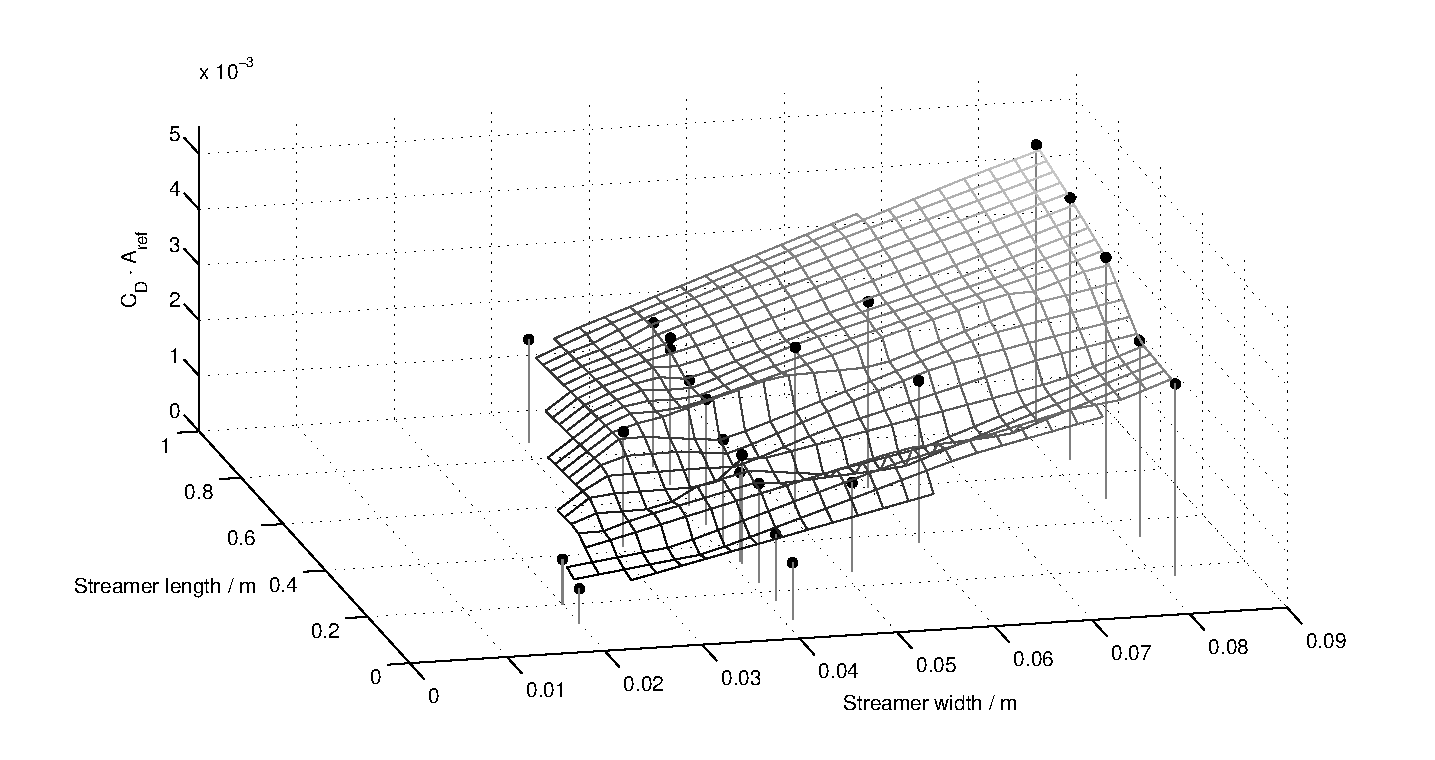
\epsfig{file=figures/experimental/streamerCDvsWL,width=155mm}
\caption{The normalized drag coefficient of a streamer as a function
  of the width and length of the streamer.  The points are the
  measured values and the mesh is cubically interpolated between the
  points.}
\label{fig-streamer-CD-vs-shape}
\end{figure}


\begin{figure}[p]
\centering
\hspace*{-7mm}
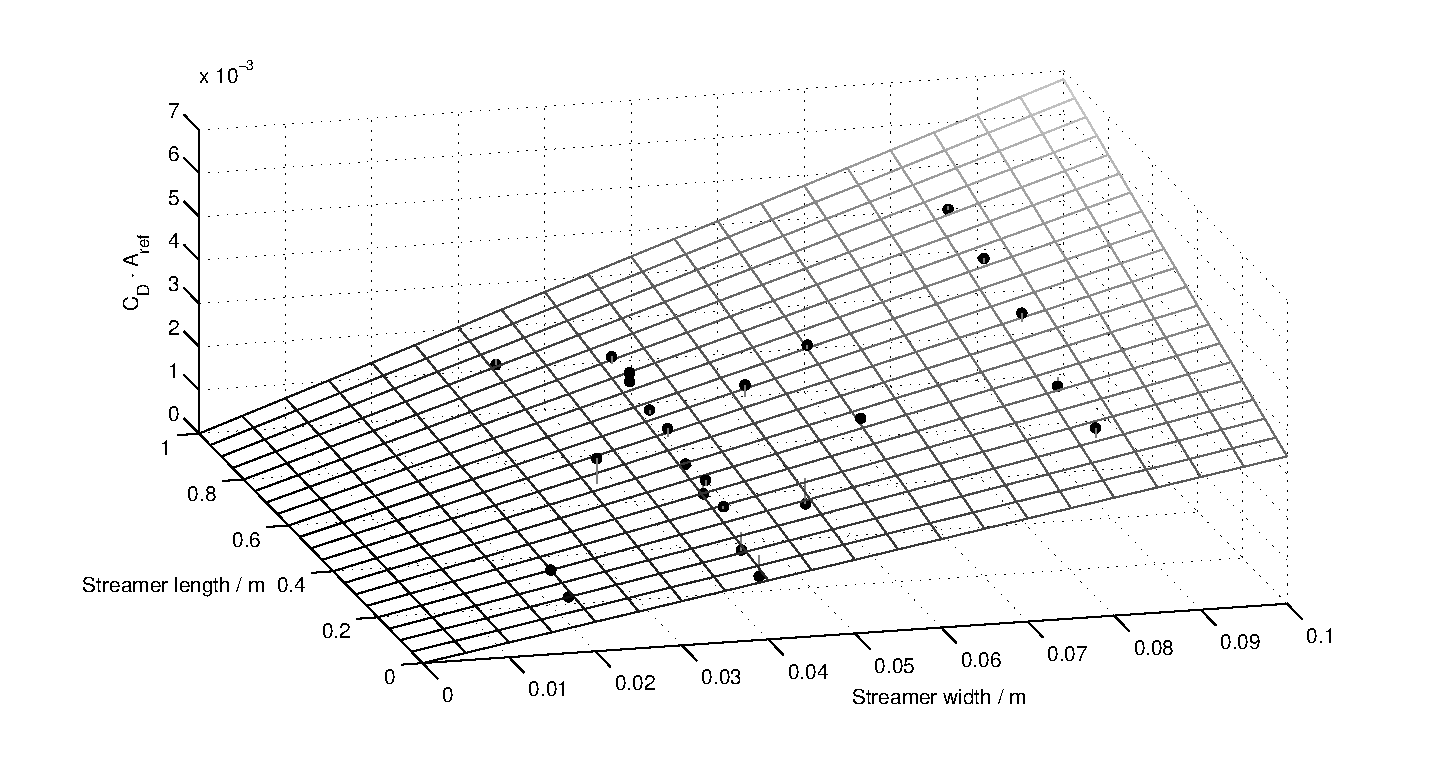
\epsfig{file=figures/experimental/streamerCDvsWLestimate,width=155mm}
\caption{Estimated and measured normalized drag coefficients of a
  streamer as a function of the width and length of the streamer.  The
  lines from the points lead to their respective estimate values.}
\label{fig-streamer-shape-estimate}
\end{figure}



Figure~\ref{fig-streamer-CD-vs-shape} presents the normalized drag
coefficient as a function of the streamer width and length for a fixed
material of $\rm80~g/m^2$ polyethylene plastic.  It was noticed that
for a specific streamer length, the normalized drag coefficient was
approximately linear with the width,
%
\begin{equation}
C_D \cdot \Aref = k\cdot w,
\label{eq-streamer-first-approx}
\end{equation}
%
where $w$ is the width and $k$ is dependent on the streamer length.
The slope $k$ was found to be approximately linear with
the length of the streamer, with a linear regression of
%
\begin{equation}
k = 0.034 \cdot (l+\rm 1~m).
\label{eq-streamer-second-approx}
\end{equation}
%
Substituting equation (\ref{eq-streamer-second-approx}) into
(\ref{eq-streamer-first-approx}) yields
%
\begin{equation}
C_D \cdot \Aref = 0.034 \cdot (l+{\rm 1~m})\cdot w
\label{eq-streamer-estimate}
\end{equation}
%
or using $\Aref = wl$
%
\begin{equation}
C_D = 0.034 \cdot \frac{l+\rm 1~m}{l}.
\label{eq-streamer-shape-estimate}
\end{equation}


The estimate as a function of the width and length is presented in 
Figure~\ref{fig-streamer-shape-estimate} along with the measured data
points.  The lines originating from the points lead to their
respective estimate values.  The average relative error produced by
the estimate was 9.7\%.


\subsubsection*{Effect of streamer material}



The effect of the streamer material was studied by creating
$4\times40$~cm and $8\times48$~cm streamers from various household
materials commonly used in streamers.  The tested materials were
polyethylene plastic of various thicknesses, cellophane and cr�pe
paper.  The properties of the materials are listed in
Table~\ref{table-streamer-materials}. 


Figure~\ref{fig-streamer-material} presents the normalized drag
coefficient as a function of the material thickness and surface
density.  It is evident that the thickness is not a good
parameter to characterize the drag of a streamer.  On the other hand,
the drag coefficient as a function of surface density is nearly
linear, even including the cr�pe paper.  While it is not as
definitive, both lines seem to intersect with the $x$-axis at
approximately  $\rm-25~g/m^2$.  Therefore the coefficient of the
$\rm80~g/m^2$ polyethylene estimated by
equation~(\ref{eq-streamer-shape-estimate}) is corrected for a
material surface density $\rho_m$ with
%
\begin{equation}
C_{D_m} = \left(\frac{\rho_m + \rm 25~g/m^2}{\rm 105~g/m^2}\right)
    \cdot C_D.
\end{equation}
%
Combining these two equations, one obtains the final empirical
equation
%
\begin{equation}
C_{D_m} = 0.034 \cdot
    \left(\frac{\rho_m + \rm 25~g/m^2}{\rm 105~g/m^2}\right) \cdot
    \left(\frac{l + 1~{\rm m}}{l}\right).
\label{eq-streamer-CD-estimate}
\end{equation}

This equation is also reasonable since it produces positive and finite
normalized drag coefficients for all values of $w$, $l$ and $\rho_m$.
However, this equation does not obey the rule-of-thumb of rocketeers
that the optimum width-to-length ratio for a streamer would be 1:10.
According to equation~(\ref{eq-streamer-estimate}), the maximum drag
for a fixed surface area is obtained at the limit $l\rightarrow0$,
$w\rightarrow\infty$.  In practice the rocket dimensions limit the
practical dimensions of a streamer, from which the 1:10 rule-of-thumb
may arise.


\subsubsection*{Equation validation}

To test the validity of the equation, several additional streamers
were measured for their drag coefficients.  These were of various
materials and of dimensions that were not used in the fitting of the
empirical formulae.  These can therefore be used as an independent
test set for validating equation~(\ref{eq-streamer-CD-estimate}).

Table~\ref{table-streamer-validation} presents the tested streamers
and their measured and estimated normalized drag coefficients.  The
results show relative errors in the range of 12--27\%.  While rather
high, they are considered a good result for estimating such a random
and dynamic process as a streamer.  Furthermore, due to the
proportionality to the square of the velocity, a 25\% error in the
normalized force coefficient translates to a 10--15\% error in the
rocket's descent velocity.  This still allows the rocket designer to
get a good estimate on how fast a rocket will descend with a
particular streamer.


\begin{figure}[p]
\centering
\parbox{70mm}{\centering
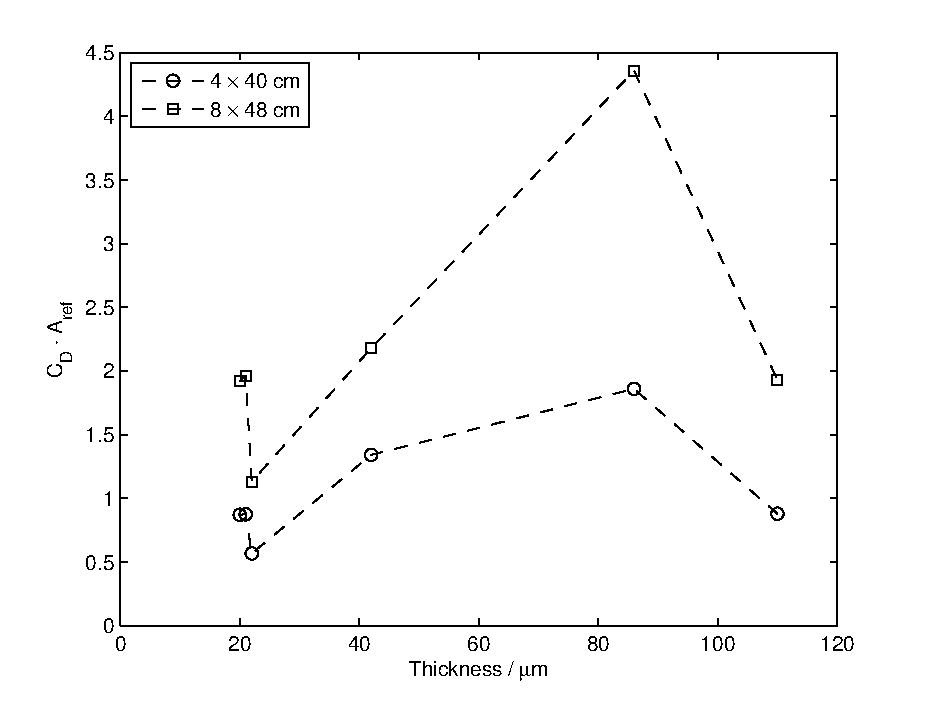
\epsfig{file=figures/experimental/streamerCDvsThickness2,width=70mm}
\\ (a)
}\parbox{70mm}{\centering
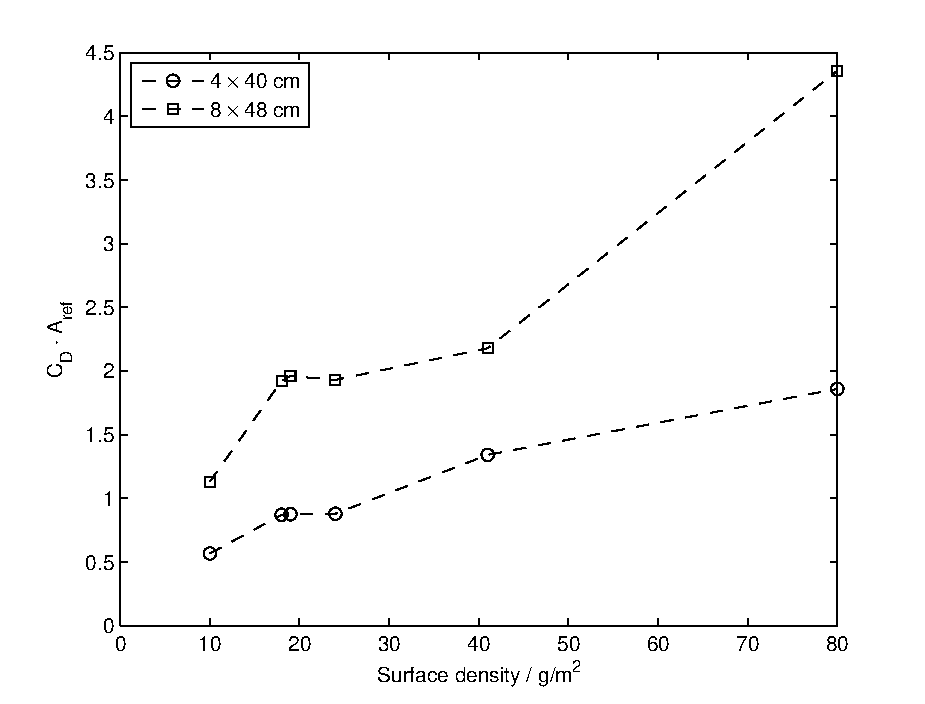
\epsfig{file=figures/experimental/streamerCDvsDensity2,width=70mm} \\ (b)}
\caption{The normalized drag coefficient of a streamer as a function
  of (a) the material thickness and (b) the material surface density.}
\label{fig-streamer-material}
\end{figure}



\begin{table}[p]
\caption{Properties of the streamer materials experimented with.}
\label{table-streamer-materials}
\begin{center}
\begin{tabular}{ccc}
\hline
Material & Thickness / \um & Density / $\rm g/m^2$ \\
\hline
Polyethylene & 21 & 19 \\
Polyethylene & 22 & 10 \\
Polyethylene & 42 & 41 \\
Polyethylene & 86 & 80 \\
Cellophane   & 20 & 18 \\
Cr�pe paper  & 110$\dagger$ & 24 \\
\hline
\end{tabular} \\
{\footnotesize $\dagger$ Dependent on the amount of pressure applied.}
\end{center}
\end{table}



\begin{table}[p]
\caption{Streamers used in validation and their results.}
\label{table-streamer-validation}
\begin{center}
\begin{tabular}{ccccccc}
\hline
Material & Width & Length & Density & Measured & Estimate & Error \\
         & m     & m      & $\rm g/m^2$ &
  \multicolumn{2}{c}{$10^{-3} (C_D\cdot\Aref)$} &  \\
\hline
Polyethylene & 0.07 & 0.21 & 21 & 0.99 & 1.26 & 27\% \\
Polyethylene & 0.07 & 0.49 & 41 & 1.81 & 2.23 & 23\% \\
Polyethylene & 0.08 & 0.24 & 10 & 0.89 & 1.12 & 26\% \\
Cellophane   & 0.06 & 0.70 & 20 & 1.78 & 1.49 & 17\% \\
Cr�pe paper  & 0.06 & 0.50 & 24 & 1.27 & 1.43 & 12\% \\
\hline
\end{tabular}
\end{center}
\end{table}

